

\begin{frame}{Contribution: Quantification sans maillage en T}
    \centering
    %\small Y. Coudert-\,-Osmont$^1$, D. Desobry$^1$, M. Heistermann$^2$, D. Bommes$^2$, N.Ray$^1$, D. Sokolov$^1$ \\
    %\tiny $^1$Inria Nancy - Grand Est, LORIA, France \\
    %\tiny $^2$University of Bern, Switzerland \\[2mm]
    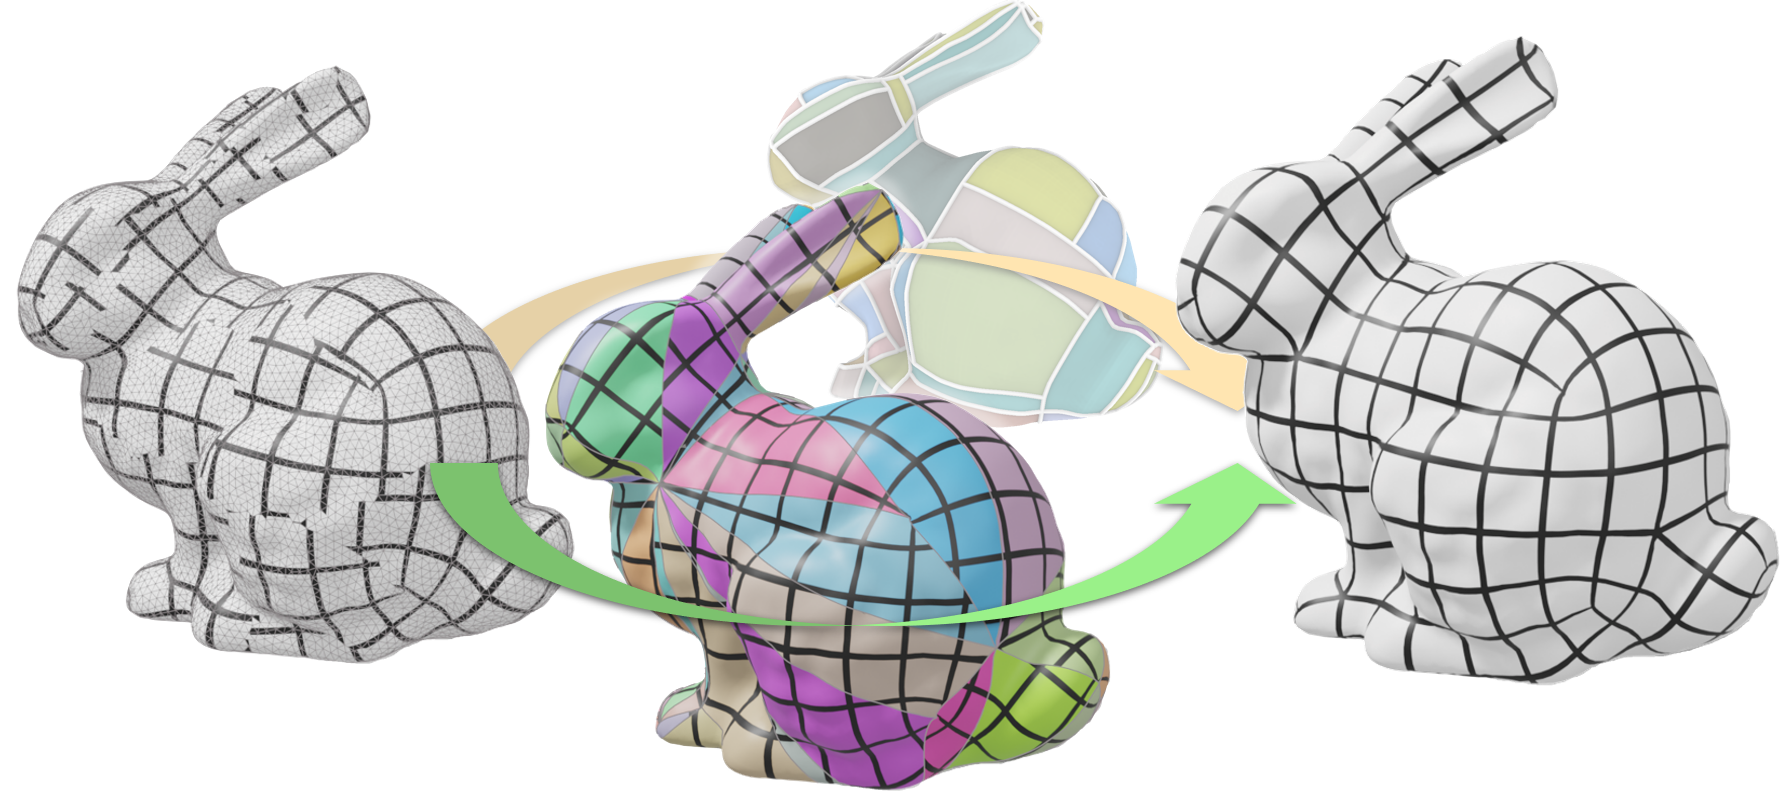
\includegraphics[width=\linewidth]{yoimg/teaser.PNG}
	\vspace{-1.5em}
	\begin{itemize}
		\item Utilisation d'une décimation du maillage triangulaire d'entrée plutôt qu'un maillage en T.
		\item Tous les sommets du maillage décimé sont des singularités.
		\item Les arêtes encodent les distances entières entre les singularités.
    \end{itemize}
\end{frame}

\begin{frame}{Contribution: Quantification sans maillage en T}
    \begin{itemize}
        \item QGP peut écraser des éléments, forçant le recalcul d'une paramétrisation bijective sous contraintes entières difficiles.\\
        \item Tous nos éléments restent valides donc la paramétrisation reste bijective et est directement utilisable.\\
        \centering
        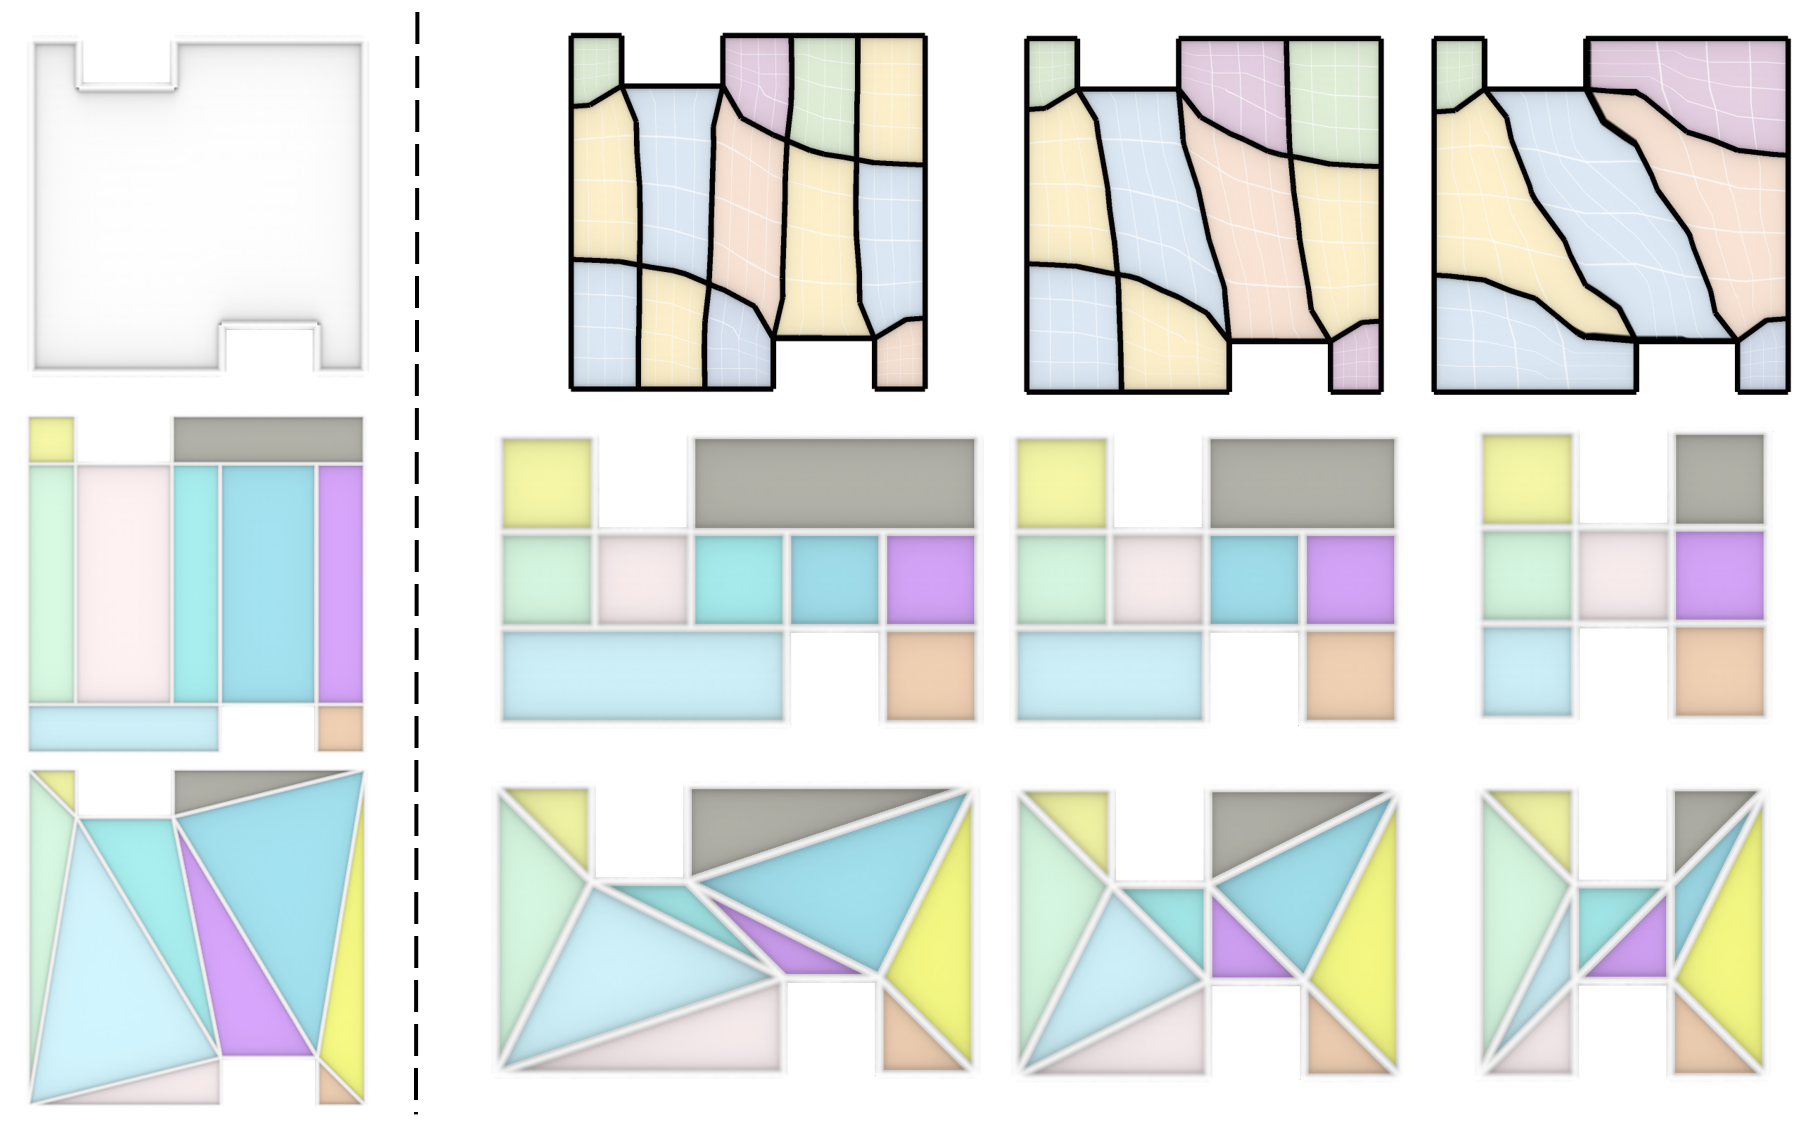
\includegraphics[width=0.75\linewidth]{yoimg/restriction.png}
    \end{itemize}
\end{frame}

\iffalse
\begin{frame}{Résultats}
    \centering
    \includegraphics[width=\linewidth]{yoimg/5_meshes.png}
\end{frame}
\fi